

%%%%%%%%%%%%%%%
%% Eigene Arbeit %%
%%%%%%%%%%%%%%%
Dieses Kapitel beinhaltet die Funktionen von der App und Website mithilfe von Anwendungsfalldiagramms und der Tabellen für die einzelnen Anwendungsfälle.
Dabei sind die Anwendungsfälle durch die Muss- und Soll-Features definiert. 

%%%%%%%%%%%%%%%
%% Anwendungsfall 1 %%
%%%%%%%%%%%%%%%

\section{Anwendungsfalldiagramm}

\begin{figure}[H]

	\hspace{-5cm}
	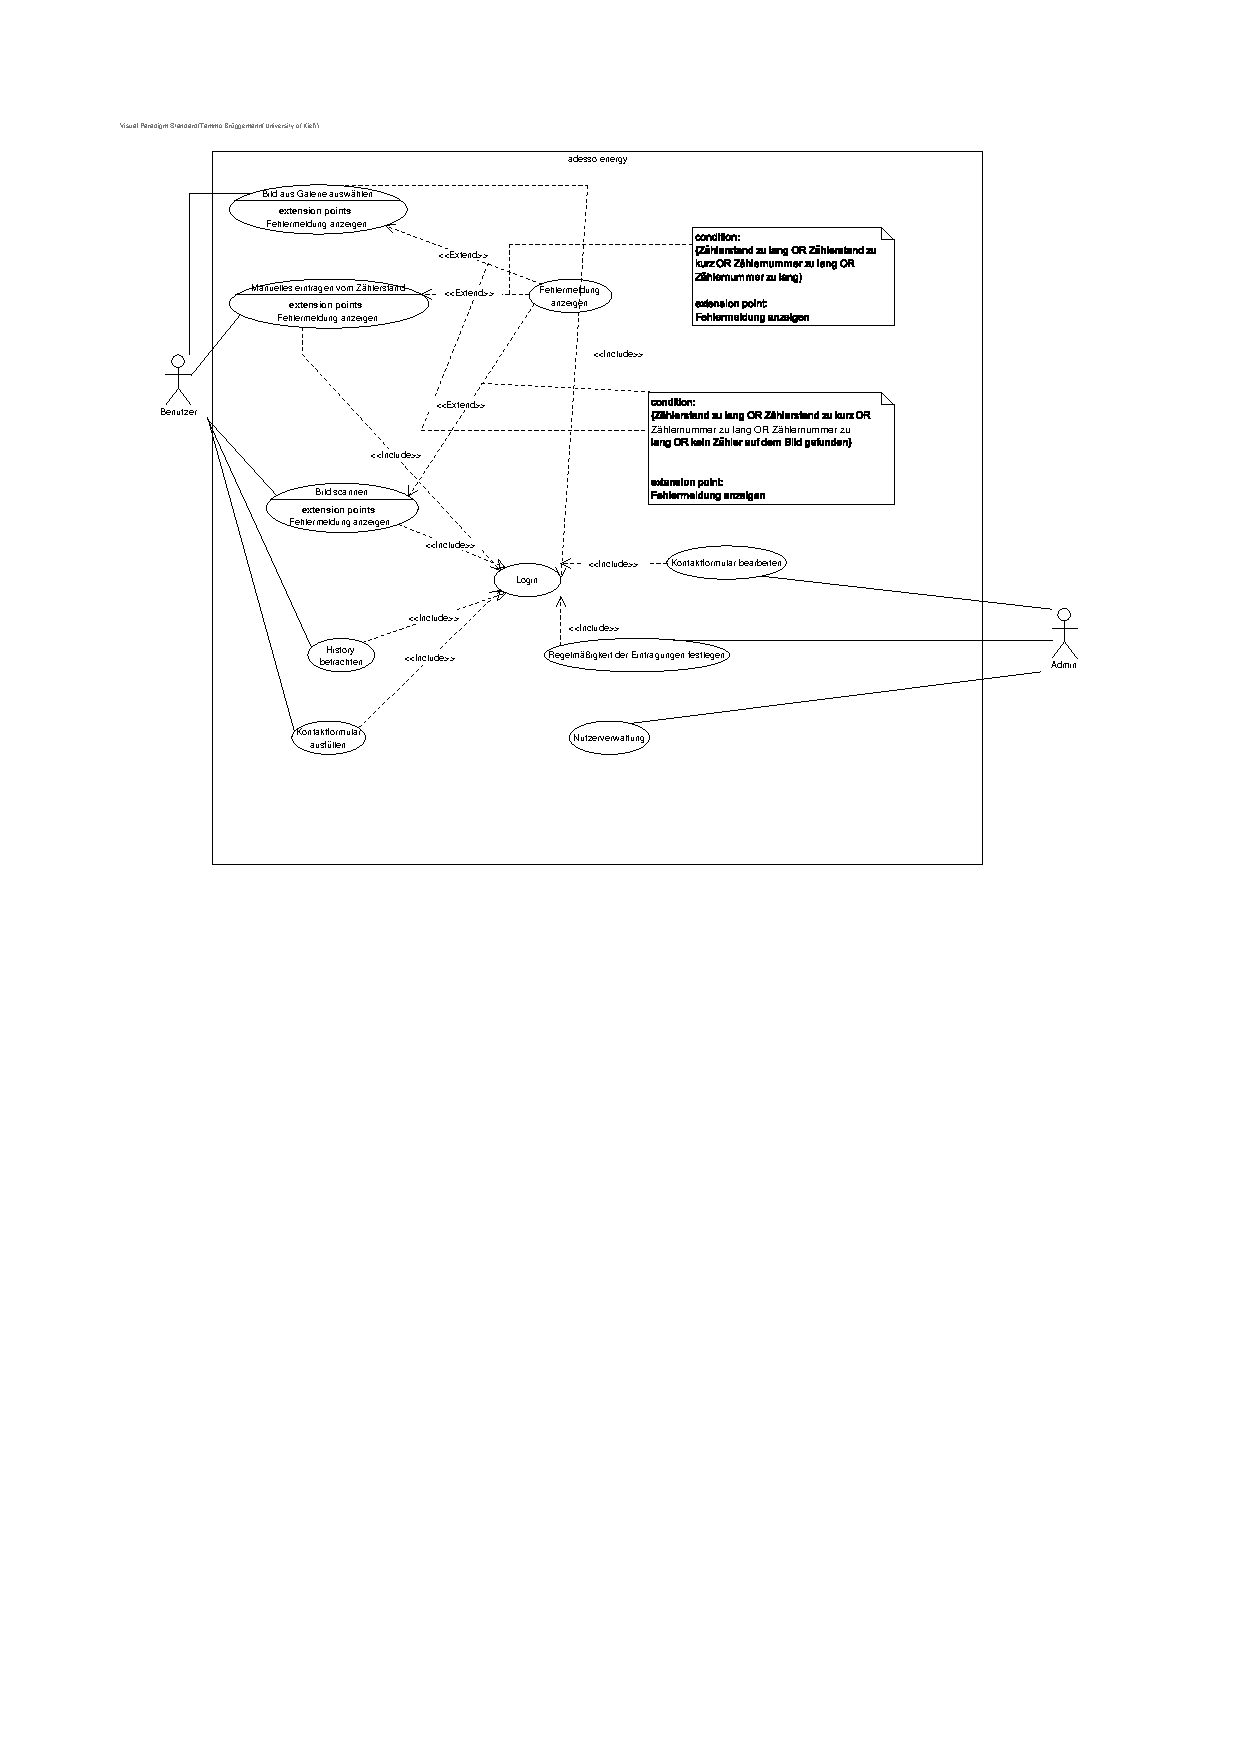
\includegraphics[width=25 cm, height = 45cm]{./img/mustCase}
%	\centering
%	\missingfigure{Anwendungsfalldiagramm - App}		
%	\caption{Anwendungsfalldiagramm - App}
%	\label{fig:anwendungsfalldiagramm-app}
\end{figure}

\newpage 

\section{Muss-Features}

\begin{figure}[H]
	\centering
	\begin{tabularx}{\textwidth}{ X | X }
		\textbf{Anwendungsfall ID} & M1 \\ \hline
		\textbf{Anwendungsfallname} & Bild hochladen  - Foto \\ \hline
		\textbf{Initiierender Akteur} & Benutzer \\ \hline
		\textbf{Weitere Akteure} & - \\ \hline
		\textbf{Kurzbeschreibung} & Benutzer macht in der App ein Foto und lädt dieses hoch.   \\ \hline
		\textbf{Vorbedingungen} & 
		\begin {itemize}
			\item Eingeloggt sein. 
			\item Hauptbildschirm geöffnet.
			\item Auf Kamera FAB gedrückt.
		\end{itemize} \\ \hline
		\textbf{Nachbedingungen} & Bei Erfolg: Zählerstand wurde erkannt und eingetragen. \\ \hline
		\textbf{Ablauf} &
		\begin{enumerate}
			\item Benutzer macht Foto.
			\item Benutzer bestätigt das Senden des Fotos.
			\item Azure wertet Bild aus.
			\item Erkannte Zählernummer und Zählerstand werden angezeigt.
			\item Benutzer bestätigt Korrektheit der Zählernummer und des Zählerstandes.
		\end{enumerate} \\ \hline
		\textbf{Alternative} &
		\begin{enumerate}
			\item Benutzer macht Foto.
			\item Benutzer bestätigt das Senden des Fotos.
			\item Azure wertet Bild aus.
			\item Erkannte Zählernummer und Zählerstand werden angezeigt.
			\item Benutzer bricht Aktion ab.
		\end{enumerate} \\ &
		\begin{enumerate}
			\item Benutzer macht Foto.
			\item Benutzer bestätigt das Senden des Fotos.
			\item Azure wertet Bild aus.
			\item Erkannte Zählernummer und Zählerstand werden angezeigt.
			\item Benutzer verändert Eingabe manuell.
		\end{enumerate} \\


	\end{tabularx}
\end{figure}

\begin{figure}[H]
	\centering
	\begin{tabularx}{\textwidth}{ X | X }
	 \hline
		\textbf{Ausnahme} &
		\begin{enumerate}
			\item Benutzer macht Foto.
			\item Benutzer bestätigt das Senden des Fotos.
			\item Azure wertet Bild aus.
			\item Fehler beim Auslesen der Zählernummer oder des Zählerstandes.
			\item $\lbrack$ Use-Case: Fehlermeldung anzeigen $\rbrack$
		\end{enumerate} \\ &
		\begin{enumerate}
			\item Benutzer macht Foto.
			\item Benutzer bestätigt das Senden des Fotos.
			\item Azure wertet Bild aus.
			\item Zählernummer und Zählerstand wurden erkannt, aber mindestens einer der beiden Werte ist unzulässig. (falsches Format)
			\item $\lbrack$ Use-Case: Fehlermeldung anzeigen $\rbrack$
		\end{enumerate} \\  &
		\begin{enumerate}
			\item Benutzer macht Foto.
			\item Benutzer bestätigt das Senden des Fotos.
			\item Es liegt ein Serverfehler vor.
			\item App zeigt eine 'Bitte versuche es nochmal'-Meldung.
		\end{enumerate} \\  &
		\begin{enumerate}
			\item Benutzer macht Foto.
			\item Benutzer bestätigt das Senden des Fotos.
			\item Benutzer hat keine Internetverbindung.
			\item App zeigt eine 'Du bist offline'-Meldung.
		\end{enumerate} \\ \hline
		\textbf{Benutzte Anwendungsfälle} & Fehlermeldung angezeigen \\ \hline
		\textbf{Spezielle Anforderungen} & - \\ \hline
		\textbf{Annahmen} & -
	\end{tabularx}
	\caption{Anwendungsfall Bild hochladen - Foto - M1}
	\label{fig:anwendungsfall-server-tabelle-xx-1}
\end{figure}

\newpage

\begin{figure}[H]
	\centering
	\begin{tabularx}{\textwidth}{ X | X }
		\textbf{Anwendungsfall ID} & M2 \\ \hline
		\textbf{Anwendungsfallname} & Zählerstand manuell eingeben. \\ \hline
		\textbf{Initiierender Akteur} & Benutzer \\ \hline
		\textbf{Weitere Akteure} & - \\ \hline
		\textbf{Kurzbeschreibung} & Benutzer hat, neben dem Abfotografieren des Zählerstandes, auch noch die Möglichkeit den Zählerstand manuell einzugeben.  \\ \hline
		\textbf{Vorbedingungen} & 
		\begin {itemize}
			\item Eingeloggt sein. 
			\item Hauptbildschirm geöffnet.
			\item Zähler auswählen.
			\item Auf Button 'Neue manuelle Eingabe' drücken.
		\end{itemize}\\ \hline
		\textbf{Nachbedingungen} & Bei Erfolg: Zählerstand wurde eingetragen.  \\ \hline
		\textbf{Ablauf} &
		\begin{enumerate}
			\item Benutzer überprüft ob angezeigte Zählernummer mit der Zählernummer des ausgewählten Zählers übereinstimmt.
			\item Benutzer gibt Zählerstand ein.
			\item Benutzer bestätigt Zählerstand.
		\end{enumerate} \\ \hline
		\textbf{Alternative} &
		\begin{enumerate}
			\item Benutzer überprüft ob angezeigte Zählernummer mit der Zählernummer des ausgewählten Zählers übereinstimmt.
			\item Benutzer bricht Aktion ab.
		\end{enumerate} \\ \hline
		\textbf{Ausnahme} &
		\begin{enumerate}
			\item Benutzer überprüft ob angezeigte Zählernummer mit der Zählernummer des ausgewählten Zählers übereinstimmt.
			\item Benutzer gibt Zählerstand ein.
			\item Benutzer bestätigt Zählerstand.
			\item Zählerstand ist unzulässig. (falsches Format)

			\item 'Dieser Wert ist unzulässig. Bitte erneut eingeben'-Meldung wird angezeigt. 
 			\item $\lbrack$ Use-Case: Zählerstand manuell eingeben - App $\rbrack$
		\end{enumerate} \\


	\end{tabularx}
\end{figure}

\begin{figure}[H]
	\centering
	\begin{tabularx}{\textwidth}{ X | X }
	\hline
	\textbf{Ausnahme} \ (forts.)&
		\begin{enumerate}
			\item Benutzer überprüft ob angezeigte Zählernummer mit der Zählernummer des ausgewählten Zählers übereinstimmt.
			\item Benutzer gibt Zählerstand ein.
			\item Benutzer bestätigt Zählerstand.
			\item Es liegt ein Serverfehler vor.
			\item Die App zeigt eine 'Bitte versuche es nochmal'-Meldung. 
			\item $\lbrack$ Use-Case: Zählerstand manuell eingeben - App $\rbrack$
		\end{enumerate} \\  &
		\begin{enumerate}
			\item Benutzer überprüft ob angezeigte Zählernummer mit der Zählernummer des ausgewählten Zählers übereinstimmt.
			\item Benutzer gibt Zählerstand ein.
			\item Benutzer bestätigt Zählerstand.
			\item Benutzer hat keine Internetverbindung.
			\item Die App zeigt eine 'Du bist offline'-Meldung.
		\end{enumerate}  \\ \hline
		\textbf{Benutzte Anwendungsfälle} & Zählerstand manuell eingeben - App \\ \hline
		\textbf{Spezielle Anforderungen} & - \\ \hline
		\textbf{Annahmen} & -
	\end{tabularx}
	\caption{Anwendungsfall Zählerstand manuell eingeben - M2}
	\label{fig:anwendungsfall-server-tabelle-xx-1}
\end{figure}

\newpage

\begin{figure}[H]
	\centering
	\begin{tabularx}{\textwidth}{ X | X }
		\textbf{Anwendungsfall ID} & M3 \\ \hline
		\textbf{Anwendungsfallname} & Fehlermeldung anzeigen \\ \hline
		\textbf{Initiierender Akteur} & Benutzer \\ \hline
		\textbf{Weitere Akteure} & - \\ \hline
		\textbf{Kurzbeschreibung} & Falls beim Auslesen eines Bildes ein Problem auftritt, wird dem Benutzer eine Fehlermeldung angezeigt.   \\ \hline
		\textbf{Vorbedingungen} & 
		\begin {itemize}
			\item Eingeloggt sein. 
			\item Hauptbildschirm geöffnet.
			\item Bild wurde hochgeladen.
			\item Azure konnte Bild nicht auswerten.
		\end{itemize}\\ \hline
		\textbf{Nachbedingungen} & - \\ \hline
		\textbf{Ablauf} &
		\begin{enumerate}
			\item Meldung 'Scan nicht erfolgreich' wird angezeigt.
			\item Benutzer drückt auf 'Neuer Scan".
			\item $\lbrack$ Use-Case: Bild hochladen - Foto $\rbrack$
		\end{enumerate} \\ \hline
		\textbf{Alternative} & 
		\begin{enumerate}
			\item Meldung 'Scan nicht erfolgreich' wird angezeigt.
			\item Benutzer drückt auf 'Abbrechen'.
			\item Benutzer ist wieder auf Startbildschirm.
		\end{enumerate} \\ \hline
		\textbf{Ausnahme} & -   \\ \hline
		\textbf{Benutzte Anwendungsfälle} & Bild hochladen - Foto \\ \hline
		\textbf{Spezielle Anforderungen} & - \\ \hline
		\textbf{Annahmen} & -
	\end{tabularx}
	\caption{Anwendungsfall Fehlermeldung anzeigen - M3}
	\label{fig:anwendungsfall-server-tabelle-xx-1}
\end{figure}

\newpage

\begin{figure}[H]
	\centering
	\begin{tabularx}{\textwidth}{ X | X }

		\textbf{Anwendungsfall ID} & M4 \\ \hline
		\textbf{Anwendungsfallname} & Zähler hinzufügen. \\ \hline
		\textbf{Initiierender Akteur} & Admin \\ \hline
		\textbf{Weitere Akteure} & - \\ \hline
		\textbf{Kurzbeschreibung} & Admin hat die Möglichkeit jedem Benutzer neue Zähler hinzuzufügen.   \\ \hline
		\textbf{Vorbedingungen} & 
		\begin {itemize}
			\item Benutzer ist registriert. 
			\item Admin ist auf der Website eingeloggt.
			\item Admin wählt Account des Benutzers aus.
			\item Admin wählt die Funktion einen neuen Zähler für diesen Benutzer hinzuzufügen aus.
		\end{itemize}\\ \hline
		\textbf{Nachbedingungen} & Bei Standardablauf: Der Account des Benutzers besitzt einen neuen Zähler. \\ \hline
		\textbf{Ablauf} &
		\begin{enumerate}
			\item Admin wählt die Art des hinzugefügten Zählers aus.
			\item Admin gibt die Zählernummer des Zählers ein.
			\item Admin bestätigt die Zählernummer.
			\item Admin gibt den aktuellen Zählerstand des Zählers ein.
			\item Admin bestätigt diesen.
		\end{enumerate} \\ \hline
		\textbf{Alternative} & 
		\begin{enumerate}
			\item Admin wählt die Art des hinzugefügten Zählers aus.
			\item Admin gibt die Zählernummer des Zählers ein.
			\item Admin bricht die Aktion ab.
		\end{enumerate} \\ &
	\end{tabularx}
\end{figure}

\begin{figure}[H]
	\centering
	\begin{tabularx}{\textwidth}{ X | X }
	\hline
	\textbf{Alternative} \ (forts.)&
		\begin{enumerate}
			\item Admin wählt die Art des hinzugefügten Zählers aus.
			\item Admin gibt die Zählernummer des Zählers ein.
			\item Admin bestätigt die Zählernummer.
			\item Admin gibt den aktuellen Zählerstand des Zählers ein.
			\item Admin bricht die Aktion ab.
		\end{enumerate} \\ \hline
		\textbf{Ausnahme} & 
		\begin{enumerate}
			\item Admin wählt die Art des hinzugefügten Zählers aus.
			\item Admin gibt die Zählernummer des Zählers ein.F
			\item Es liegt ein Serverfehler vor.
			\item Website zeigt eine 'Bitte versuche es nochmal'-Meldung.
		\end{enumerate} \\ &
		\begin{enumerate}
			\item Admin wählt die Art des hinzugefügten Zählers aus.
			\item Admin gibt die Zählernummer des Zählers ein.
			\item Admin bestätigt die Zählernummer.
			\item Admin gibt den aktuellen Zählerstand des Zählers ein.
			\item Es liegt ein Serverfehler vor.
			\item Website zeigt eine 'Bitte versuche es nochmal'-Meldung.
		\end{enumerate} \\ \hline
		\textbf{Benutzte Anwendungsfälle} & Bild hochladen - Foto \\ \hline
		\textbf{Spezielle Anforderungen} & - \\ \hline
		\textbf{Annahmen} & -
	\end{tabularx}
	\caption{Anwendungsfall Zähler hinzufügen - M4}
	\label{fig:anwendungsfall-server-tabelle-xx-1}
\end{figure}
\newpage

\section{Soll-Features}

\begin{figure}[H]
	\centering
	\begin{tabularx}{\textwidth}{ X | X }
		\textbf{Anwendungsfall ID} & S1 \\ \hline
		\textbf{Anwendungsfallname} & Kontaktaufnahme \\ \hline
		\textbf{Initiierender Akteur} & Benutzer \\ \hline
		\textbf{Weitere Akteure} & - \\ \hline
		\textbf{Kurzbeschreibung} & Benutzer kontaktiert den Service. \\ \hline
		\textbf{Vorbedingungen} &
		\begin {itemize}
			\item Benutzer ist eingeloggt.
			\item Hauptbildschirm ist geöffnet.
		\end{itemize}\\ \hline
		\textbf{Nachbedingungen} & Auf dem Server wurde ein Ticket erstellt. \\ \hline
		\textbf{Ablauf} &
		\begin{enumerate}
			\item Benutzer wählt im Menü auf dem Hauptbildschirm 'Kontakt' aus .
			\item Benutzer gibt sein Problem und seine Kontaktdaten ein .
			\item Benutzer drückt auf Senden.
			\item App schickt die eingegeben Daten an den Server. 
			\item Server speichert diese Daten.
		\end{enumerate} \\ \hline
		\textbf{Alternative} &
		\begin{enumerate}
			\item Benutzer wählt im Menü auf dem Hauptbildschirm 'Kontakt' aus .
			\item Benutzer gibt sein Problem und seine Kontaktdaten ein .
			\item Benutzer bricht die Aktion ab.
		\end{enumerate}  \\ \hline
		\textbf{Ausnahme} &
		\begin{enumerate}
			\item Benutzer wählt im Menü auf dem Hauptbildschirm 'Kontakt' aus.
			\item Benutzer gibt sein Problem und seine Kontaktdaten ein.
			\item Benutzer drückt auf Senden.
			\item Benutzer hat keine Internetverbindung.
			\item App zeigt eine 'Du bist offline' -Meldung.
		\end{enumerate} 
	\end{tabularx}
\end{figure}

\begin{figure}[H]
	%\centering
	\begin{tabularx}{\textwidth}{ X | X }
	\hline
	\textbf{Ausnahme} \ (forts.)&
		\begin{enumerate}
			\item Benutzer wählt im Menü auf dem Hauptbildschirm 'Kontakt' aus. 
			\item Benutzer gibt sein Problem und seine Kontaktdaten ein.
			\item Benutzer drückt auf Senden.
			\item App schickt die eingegeben Daten an den Server.
			\item Es liegt ein Serverfehler vor.
			\item App zeigt eine 'Bitte versuche es nochmal' -Meldung.
		\end{enumerate} \\ \hline
		\textbf{Benutzte Anwendungsfälle} & - \\ \hline
		\textbf{Spezielle Anforderungen} & - \\ \hline
		\textbf{Annahmen} & -
	\end{tabularx}
	\caption{Zählerstand manuell eingeben - S1.}
	\label{fig:anwendungsfall-server-tabelle-xx-1}
\end{figure}
\begin{figure}[H]
	\centering
	\begin{tabularx}{\textwidth}{ X | X }
		\textbf{Anwendungsfall ID} & S2 \\ \hline
		\textbf{Anwendungsfallname} & Bild Hochladen - Galerie \\ \hline
		\textbf{Initiierender Akteur} & Benutzer \\ \hline
		\textbf{Weitere Akteure} & - \\ \hline
		\textbf{Kurzbeschreibung} & Benutzer lädt ein Foto aus der Galerie zur Analyse hoch. \\ \hline
		\textbf{Vorbedingungen} &
		\begin {itemize}
			\item Benutzer ist eingeloggt.
			\item Hauptbildschirm ist geöffnet.
			\item Auf Galerie FAB gedrückt.
		\end{itemize}\\ \hline
		\textbf{Nachbedingungen} & Zählerstand wurde erkannt und eingetragen. \\ \hline
		\textbf{Ablauf} &
		\begin{enumerate}
			\item Benutzer wählt Foto aus Galerie aus.
			\item Benutzer bestätigt das Senden des Fotos. 
			\item Azure wertet Bild aus.
			\item Erkannte Zählernummer und Zählerstand werden angezeigt. 
			\item Benutzer bestätigt Korrektheit der Zählernummer und des Zählerstandes.
		\end{enumerate} \\ \hline
		\textbf{Alternative} & 
		\begin{enumerate}
			\item Benutzer wählt Foto aus Galerie aus .
			\item Benutzer bestätigt das Senden des Fotos.
			\item Azure wertet Bild aus. 
			\item Erkannte Zählernummer und Zählerstand werden angezeigt. 
			\item Benutzer bricht Aktion ab. 
		\end{enumerate}
		\\&
		\begin{enumerate}
			\item Benutzer wählt Foto aus Galerie aus.
			\item Benutzer bestätigt das Senden des Fotos. 
			\item Azure wertet Bild aus.
			\item Erkannte Zählernummer und Zählerstand werden angezeigt. 
			\item Benutzer verbessert Eingabe manuell.
		\end{enumerate} \\
	\end{tabularx}
\end{figure}
\begin{figure}[H]
	%\centering
	\begin{tabularx}{\textwidth}{ X | X } \hline
		\textbf{Ausnahme} &
		\begin{enumerate}
			\item Benutzer wählt Foto aus Galerie aus.
			\item Benutzer bestätigt das Senden des Fotos.  
			\item Azure wertet Bild aus.
			\item Fehler beim Auslesen der Zählernummer, des Zählerstandes oder des Zählertyps. 
			\item $\lbrack$ Use-Case: Fehlermeldung wird angezeigt $\rbrack$ 
		\end{enumerate} 
		\\&
		\begin{enumerate}
			\item Benutzer wählt Foto aus Galerie aus.
			\item Benutzer bestätigt das Senden des Fotos. 
			\item Azure wertet Bild aus. 
			\item Zählernummer, Zählerstand und Zählertyp wurden erkannt, aber die Werte sind unzulässig. (falsches Format) 
			\item $\lbrack$ Use-Case: Fehlermeldung wird angezeigt $\rbrack$ 
		\end{enumerate}  
		\\&
		\begin{enumerate}
			\item Benutzer wählt Foto aus Galerie aus.
			\item Benutzer bestätigt das Senden des Fotos. 
			\item Es liegt ein Serverfehler vor. 
			\item App zeigt eine ’Bitte versuche es nochmal’-Meldung. 
		\end{enumerate}
		\\&
		\begin{enumerate}
			\item Benutzer wählt Foto aus Galerie aus.
			\item Benutzer bestätigt das Senden des Fotos.
			\item Benutzer hat keine Internetverbindung. 
			\item App zeigt eine ’Du bist offline’- Meldung.
		\end{enumerate} \\ \hline
		\textbf{Benutzte Anwendungsfälle} & - \\ \hline
		\textbf{Spezielle Anforderungen} & - \\ \hline
		\textbf{Annahmen} & - \\ \hline
	\end{tabularx}
	\caption{Zählerstand manuell eingeben - S2.}
	\label{fig:anwendungsfall-server-tabelle-xx-1}
\end{figure}

\newpage

\begin{figure}[H]
	\centering
	\begin{tabularx}{\textwidth}{ X | X }
		\textbf{Anwendungsfall ID} & S3 \\ \hline
		\textbf{Anwendungsfallname} & Push-Nachrichten \\ \hline
		\textbf{Initiierender Akteur} & Server \\ \hline
		\textbf{Weitere Akteure} & Benutzer \\ \hline
		\textbf{Kurzbeschreibung} & Benutzer bekommt eine Push-Benachrichtigung. \\ \hline
		\textbf{Vorbedingungen} & - \\ \hline
		\textbf{Nachbedingungen} & Benutzer hat eine Push-Benachrichtigung erhalten. \\ \hline
		\textbf{Ablauf} & Server sendet eine Push-benachrichtigung. \\ \hline
		\textbf{Alternative} & - \\ \hline
		\textbf{Ausnahme} &
		\begin{itemize}
			\item Benutzer hat kein Netz.
			\item Benachrichtigung wird später geschickt.
		\end{itemize} \\ \hline
		\textbf{Benutzte Anwendungsfälle} & - \\ \hline
		\textbf{Spezielle Anforderungen} & - \\ \hline
		\textbf{Annahmen} & -
	\end{tabularx}
	\caption{Zählerstand manuell eingeben - S3.}
	\label{fig:anwendungsfall-server-tabelle-xx-1}
\end{figure}